\documentclass{sig-alternate}
\usepackage{fontspec}
\usepackage{xunicode}
\usepackage{amsmath}
%\usepackage{amsthm}
\usepackage{graphicx}
\date{}
%\newtheoremstyle{dense}{10pt}{40pt}
%\theoremstyle{dense}
%\theoremstyle{remark}
\newtheorem{lemma}{Lemma}
\newcommand{\tighten}{\setlength{\itemsep}{1pt}\setlength{\parskip}{0pt}\setlength{\parsep}{0pt}}
\newenvironment{tightitem}{
\begin{itemize}
  \setlength{\itemsep}{1pt}
  \setlength{\parskip}{0pt}
  \setlength{\parsep}{0pt}}{\end{itemize}
}

\begin{document}

\conferenceinfo{WikiSym}{'10, July 7-9, 2010, Gdansk, Poland}
\CopyrightYear{2010}
\crdata{978-1-4503-0056-8/10/07}

\title{Deep Hypertext with Embedded Revision Control Implemented in Regular Expressions}

\author{Victor Grishchenko \\ \small Delft University of Technology, Ural State University \\ {\tt victor.grishchenko@gmail.com} }

\maketitle

\begin{abstract}
While text versioning was definitely a part of the original
hypertext concept~\cite{nls,literary,hyp-ed-sys},
it is rarely considered in this context today.
Still, we know that revision control underlies the most exciting
social co-authoring projects of today's Internet, namely the
Wikipedia and the Linux kernel. With an intention to adapt the
advanced revision control technologies and practices to the
conditions of the Open Web, the paper reconsiders some obsolete
assumptions and develops a new versioned text format perfectly
processible with standard regular expressions (PCRE~\cite{pcre}).
The resulting \emph{deep} hypertext model extends the linking
concept from inter-document associations to intra-document
dependencies and evolution. As the most promising consequence,
it allows distributed and real-time revision control in the Open
Web, i.e. co-evolution and mutation exchange among multiple
competing versions of the same text. 

\end{abstract}

\category{I.7.1}{Document and text processing}{Document and Text Editing}[Version control]
\category{H.5}{Information interfaces and presentation}{Hypertext/Hypermedia}

\section{Rationale}

Historically, the object model of the World Wide Web is a graph of pages connected by unidirectional links.
In this context, the value of a link is an association between two pages.
Evolution of a single page is an obstacle as it potentially breaks links; it is out of the model’s scope.
While a web of pages may scale indefinitely, our perception can not. 
Normally, we resort to a search engine ranking millions of pages to cherry-pick those most relevant to us.
%During the last decade, we have also witnessed the fundamentally different
There also exists an alternative approach of fusing a multitude of contributions into a singular document which an end user is able to consume.
Thus, the user's perception is effectively scaled up.
The most notable example of the approach is the Wikipedia and wikis in general.
That process of knowledge fusion is inherently social and focuses on the evolution of a document, exactly the process the World Wide Web omits.

Ironically, document evolution was addressed in-depth in the original Xanadu hypertext model~\cite{literary}, albeit no convincing usecase was provided.
Currently, most of advances in document evolution and revision control are made in the context of Source Code Management (SCM).
Considering the wiki-world and Wikipedia in particular, typically the employed revision control technology is as obsolete as you can possibly get.
That is especially clear if compared to the recent developments in Distributed Revision Control Systems (DRCS) employed by the Linux kernel and other large-scale software development projects.
Another relatively new development is real-time revision control, which powers group collaboration environments. Notable examples are Etherpad, Google Docs, Google Wave.

Knowledge fusion scales our perception, but how can we scale the fusion itself?
Consider Wikipedia; it certainly faces a scalability barrier \cite{no-singularity, wp-decay}.
In case scalability issues are resolved, we may witness something even more useful and exciting, perhaps a Web-scale Wikipedia housing both general and specialized knowledge.
Probably, we may borrow some practices from the SCM field.
Indeed, all the advanced SCM techniques, such as optimistic locking, 3-way merge, branching, distributed revision control, etc, were not introduced for the art's sake.
Each technique overcomes a certain scalability barrier that have emerged once software projects became sufficiently big.
Consistently, SCM technology drifted to higher degrees of parallelism, decentralization and autonomy and the recent DRCS boom is just another example.

The objective of this work is to develop a Web-ready revision control technology which is perfectly distributed and real-time, uniting the best of both worlds.
Apart from the promise of scalability, the technology potentially improves usability/ accessibility/ availability of wikis~\cite{nahaboo} and enables new uses, such as federated wikis with social filtration of changes~\cite{www06}, or real-time brainstorming wiki (think Etherpad backed by git~\cite{git}) or simply offline use of wikis.

To give an introduction to the technical part of the problem we devote Section~\ref{sec:scm} to review the technological foundations of revision control. 
%As it was said, Wikipedia's technology is lagging 20 to 30 years behind the state of the art in the source code management field. 
In Section~\ref{sec:textile}, we proceed to the focal topic of this paper which is the adaptation of advanced revision control technologies for Open-Web hypertext versioning. As a result, we come up with a vision of \emph{deep} hypertext carrying its history, authorship attribution and internal dependencies.
The section outlines a simple hypertext storage format with embedded revision control.
Then, in Section \ref{sec:algos}, the concept is proven to be practical by implementing both basic and advanced revision control operations, mostly relying on Perl-compatible regular expressions, which are readily available not only in numerous programming languages, but even in the constrained environment of a Web browser, thanks to JavaScript.
Next, Section~\ref{sec:estim} physical/practical limitations are considered to ensure feasibility of the format and algorithms.
The format is applied to hierarchically structured texts.
Section \ref{sec:reflections} hints at some promising implications and consequences of the introduced technology.
Section~\ref{sec:conclusion} concludes.



\section{Revision control basics} \label{sec:scm}

I will first outline principles and inner workings of revision control technologies.
%\subsection{Storage}
The most basic decision and tradeoff of a revision control system is the versioned data storage format.
The simplest storage format is \emph{snapshots}: every single  version is kept in the storage.
The simplistic approach has a serious shortcoming: the space consumed by the storage tends to grow as $O(N^2)$, where $N$ is the size of the file, assuming the file grows in small increments, which is often the case.
The effect is caused by the fact that every small change causes the entire file being written all over again.
In particular, English Wikipedia (enwiki) clearly faced that problem. Their last successful regular full-history dump was made on January 2008; the next successful dump was started in January 2010 and took two months to complete~\cite{own-experience}.
Smaller pedias are still doing quite well; apparently their $O(N^2)$ is not out of bounds yet.
As an extreme example, snapshot storage is totally unacceptable for real-time version control, where changes are introduced symbol by symbol, so the $O(N^2)$ would be quite close to exactly $N^2$ of storage (1MB for 1KB of text, 100MB for 10KB etc).
An improvement over snapshots is \emph{delta}-based storage.
Delta storage keeps just some versions of a file as snapshots, the rest being stored as a sequence of deltas.
To recover a historical version, a number of deltas should be applied to a snapshot.
So far, this method is the most popular in the SCM field.
The git, for example, nominally employs snapshot storage, but older revisions are delta-compressed for storage efficiency. 
The third classic storage format is the  \emph{weave}~\cite{rcs-txt,revctrl-weave}. 
A weave contains all the pieces of a text that ever existed, in their natural order, annotated with their birth and death ``dates''.
Given a certain revision id, a weave may be scanned, so all pieces alive at that point in time will form the corresponding version of the text.
Weave is considered complex to implement; as a file format, it also suffers of high input-output overhead~\cite{bazaar-weave} as the entire weave has to be overwritten on every change.
As a consequence, it is not widely used as a storage format.
%An attempt to adapt the classic weave format for non-linear history seemingly makes it even more complex.
Still, it is often used as an interim data structure by algorithms merging concurrently introduced changes.

%\subsection{Evolution}
The storage method is closely connected to the evolution model a RCS implements.
The simplest model is a linear sequence of revisions; this is the case of Wikipedia.
Even the most antiquated RCSes use the branching model: the history is seen as a tree, where branches are eventually forked or merged back into the trunk.
Distributed revision control takes branching to the limit; the history is seen as a directed acyclic graph; every change is potentially a fork.
%different peer repositories might keep different subsets of the history.
Mass migration to non-linear development and DRCSes is the most notable trend of past years.
Linux is developed with the git, Google Code adopted Mercurial~\cite{mercurial}, and numerous open source projects head in the same direction, migrating from legacy CVS or Subversion.
The advantage of DRCS is the ability to routinely and continuously fork and merge back numerous semi-independent versions of a project.
Technically, DRCS sees every repository as an independent peer, keeping the entire project's history. The symmetric architecture minimizes client-server roundtrips, has no single point of failure or contention.
On the social side, it facilitates decentralization as well.
Fundamentally, it allows for better scalability of software development: more people doing more things at once, without causing chaos.

%\subsection{Changes}
Last but not least cornerstone of RCS design is the change serialization and propagation format.
Earlier centralized RCSes (SCCS, MS SourceSafe) employed locking to ensure exclusive access to any given file.
That made change serialization trivial: it was sufficient to mention inserted/removed parts and their \emph{positions} in the text.
But locking did not scale well, so later systems (CVS, Subversion) switched to optimistic merge of non-conflicting concurrent changes.
For the cases of no RCS, there was a practice of changesets, maintained and distributed as patches \cite{stdpatch} in parallel with the main ``upstream'' codebase.
These practices boosted the use of revision control for communication, in addition to archival. 
In presence of concurrent changes, the problem of change serialization became less trivial.
The classic \verb+patch+ utility employs a set of heuristics and combinatorial algorithms to apply changes properly; positions are always considered as approximate~\cite{patch,fraser}, every change is shipped with its \emph{context}, i.e. chunks of unchanged text before and after the changed area.
%New methods in change serialization were necessitated by the emergence of real-time revision control systems, mostly used in groupware.

Emergence of real-time groupware demanded new methods of change serialization.
An earlier example is Google Docs, which used the classic revision control techniques~\cite{diff-match-patch}, such as patches~\cite{patch} and Meyer's diff~\cite{meyers-diff}; it just invoked those operations more often, automatically.
The Google Wave project employed a new truly real-time approach derived from the previous academic work~\cite{jupiter} on Operational Transformation (OT).
Apparently, Google Docs have also switched to OT recently~\cite{own-experience}.
OT starts with the same model as the classical revision control techniques: a text is a chain of atoms, any changes are represented as insert or remove \emph{operations} at certain \emph{positions} in the text.
The problem is, once editing is done concurrently, those operations cannot be integrated easily.
The position numbering depends on previous changes and once some previous changes are concurrent and thus unknown, position numbers become inconsistent.
The OT approach applies \emph{transformations} to the mutation operations to amend the position numbers and to integrate concurrent changes consistently. The OT theory~\cite{sun-achieving} mentions three basic consistency requirements, also known as the CCI model: 
\begin{tightitem}
\item causally dependent operations are always executed in their cause-effect order (causality preservation)
\item all sites converge to the same state of text once they execute the same set of operations, independently of their order of arrival, which may vary due to concurrency (convergence)
\item the effect of executing an operation is always the originally intended effect; position shifts must not cause misapplication of operations (intention preservation)
\end{tightitem}
The only problem of OT theory is, informally, its legendary complexity, approaching that of the string theory.
Very similarly, there are numerous classes of OT flavors~\cite{ot}.
The source of OT complexity is the entangled web of interdependencies between operations, especially those concurrently introduced.
Several OT models were later found to be inconsistent; e.g. see \cite{molli-proving, woot} for an observation of the TP2 puzzle story.
The relatively recent SDT flavor is believed to be consistent even in peer-to-peer environments; in~\cite{lili-preserving} authors reference ``a 12-page formal correctness proof'' of the fact; the detailed description of SDT is 59 pages~\cite{lili-ensuring}.
Indeed, once we allow non-realtime/offline functioning, lots of concurrency and absence of any central coordinating entity, the combinatorics of OT becomes extremely poor (see Sec.~\ref{sec:ot}).
Many OT flavors resort to a single central authority to merge concurrent changes in a single consistent way; the most notable example is Google Wave's OT.
The inner workings of Wave OT are not known yet, the only released whitepaper~\cite{waveot} gives a very general overview of the algorithms (see Sec.~\ref{sec:waveot}).

At this point, it makes sense to reconsider basic assumptions that shaped the classic technologies of revision control, as those assumptions seem weak in the present circumstances. 
First of all, that atoms are necessarily addressed by their positions in a text.
The method introduces numerous unpleasant consequences, as position numbers in a changing text are very unreliable. 
Historically, unique symbol/line identifiers were considered too complex or too expensive, albeit some recent proposals involve them~\cite{woot,logoot}.
Second classic assumption to be questioned is the separation of a revision control program from an editor program, so the former only accesses snapshots of the text made by the latter.
The revision control program is supposed to run the longest common subsequence algorithm~\cite{lcs-algo} to recover what actually happened to the text.
This unfortunate loss of knowledge in-between two applications is avoided by Web-based real-time editing applications, as they instantly know every keystroke made by the user.
It is likely to be avoidable in many other cases; e.g. once revision control code is easily embeddable.
The third assumption is the line-based tracking of changes. Single symbols lacked unique ``identity'' to be used as atoms. Also, finer-grained atoms increased the running time of key algorithms  that had super-linear complexity.
%Also, classic algorithms had super-linear complexity and line-based control conveniently reduced the $N$ of atoms.
But, once we move from plain text and source code to richer formats, ``a line'' is no longer natural nor convenient.
If small changes are prevalent, which is the case with real-time systems, line-based tracking inflates overhead.
The ``old'' Google Docs, for example, worked with symbol-atoms, possibly using line-atoms as an optimization.


\section {Adaptation}   \label{sec:textile}

Back to the objective of adapting advanced version control technology to the Open Web, let's consider the requirements and the corresponding problems of the current technologies (Sec.~\ref{sec:req}). 
In the same Section, I will outline the proposed solutions.
In Sec.~\ref{sec:data}, I will introduce three basic data structures used in this work: a variant of weave, a variant of vector timestamp (weft), and a kind of operation log (yarn). Data structures are string-based, processed with regular expressions (i.e. stackless algorithms). That guarantees they are \emph{simple} in the very formal sense.
In Sec.~\ref{sec:siblord}, I address the case of concurrent changes and prove the CCI correctness.

\subsection {Requirements} \label{sec:req}
First of all, revision control is normally implemented in complex standalone software.
Although there are JavaScript implementations of basic algorithms such as Fraser's diff-match-patch~\cite{diff-match-patch}, those are heavyweight heuristic-rich combinatorial algorithms and, frankly, better be optimized out completely.
I will target a set of version control algorithms entirely implementable in linear-complexity regular expressions without any combinatorial part.

Second, both to exclude position-dependent logic and to allow for truly real-time revision control, I will represent all mutations at single-symbol granularity, each symbol being uniquely identified.
Such uniquely identified symbols are named \emph{atoms}.

Third, the problem of merging concurrent changes must be resolved in a simple automatic way, without any user intervention.
Definitely, \emph{semantically} correct merge of changes is impossible in principle; semantically correct concurrent changes, being merged cleanly in the technical sense, still may produce a semantically incorrect result.
There are no way to prevent that from happening, apart from employing some sort of artificial intelligence.
Thus, real-world RCSes focus on technically correct merge, resorting to human intervention in case some heuristics detect a dangerous situation (e.g. concurrent changes to the same line).
We will focus on technically correct and predictable way of merging, additionally emphasizing the convergence requirement.

Fourth, versioned data formats tend to be quite complex.
We will use string-based formats, composed of equal-width fields; those are effectively arrays of tuples.
Strings and regular expressions belong to the standard toolkit of every high-level language (except probably Erlang); they are highly-optimized and work at nearly-native speeds at worst.
In some browsers \cite{irregex,wrec}, regexes are directly compiled into machine code.

\subsection{Data structures}	\label{sec:data}

\newcommand{\aum}{{\fontspec{Devanagari MT}\selectfont ॐ}}
\newcommand{\eoa}{{\fontspec{Geeza Pro}\selectfont ۝}}
\newcommand{\bsp}{{\fontspec{Apple Symbols} ⌫}}
\newcommand{\cnc}{{\fontspec{Apple Symbols} ⌦}}
\newcommand{\zero}{{\fontspec{Apple Symbols} ⌀}}

Our basic data structure will be a \emph{yarn}\footnote{In this discipline, many classic terms, such as patch, weave or string, have textile connotations. Thus, I introduce terms ``yarn'' and ``weft'' in accordance with the tradition. A confused reader may substitute that for ``user's contributed symbols vector'' and ``Fidgean vector timestamp'' resp.}, an append-only sequence of atoms (i.e. symbols) introduced to a single page by a single author.
A yarn is identified by its URL.
Every symbol-atom in a yarn is identified with its offset, denoted with a single Unicode char.
``Our'' yarn is our reference point; other yarns belong to other authors.
Thus our yarn has an associated reference \emph{frame}, which is an append-only list of peer yarn URLs. The first entry on the list is ``our'' yarn URL.
Each peer yarn is thus identified by its offset in the frame list, also denoted with a single Unicode char.
Thus, a full identifier of an atom consists of two chars: one char for its yarn, another for its offset within the yarn.
An identifier is only effective within its frame.
So, at this point we may use three forms of tuples to encode an atom. The simplest 1-form contains the actual character only, e.g. ``T'' in Fig.~\ref{fig:ds}. The 2-form contains its id, i.e. the yarn and the offset: ``a1''. The 3-form contains both the character and the id: ``Ta1''.
%As I stick to string-based formats, I will use Unicode chars instead of integers to mark
%Instead of numbers we will use single Unicode chars (code points).
%A yarn may reference other yarns, in case the page was co-authored by other authors besides the observer.
%This in turn creates different forms of atom encoding, such as 1-form (the symbol itself) or 3-form (a symbol and its full identifier).
%Yarn indexes used in peer yarns are supposed to be consistent with the frame of the observer (see Sec~\ref{sec:lamport} for discussion of relativistic aspects of the model).

Single symbols are linked into a text through the causality relation.
A symbol is said to be \emph{caused} by its preceding symbol at the time of insertion.
This adds three other forms: 5-form (the symbol, its own id, its causing id), 3c-form (the symbol and the causing id) and 5c-form (the same as 5-form, but the causing atom id goes first).
Further on, all data structure names will be postfixed with the the form they use, e.g. {\tt yarn3c} or {\tt atom5c}, see Fig.~\ref{fig:forms}.

\begin{figure}[t]
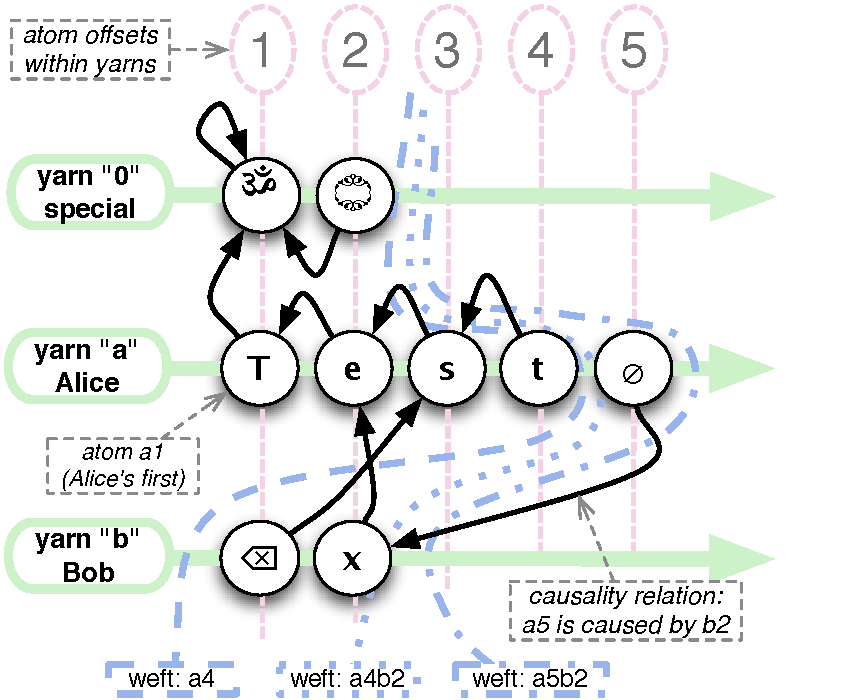
\includegraphics[width=0.49\textwidth]{feedsnweaves-5.pdf}
\caption{Yarns, wefts and weaves: Alice writes ``Test'', Bob corrects to ``Text'', Alice saves the state. \label{fig:ds} }

\resizebox{0.48\textwidth}{!}{
\begin{tabular}{|c|c|c|c|l|}
\hline
{\tt weft2} & {\tt weftI} & {\tt weave1} & {\tt text1} & comment\\
\hline
a4 & 4 &\aum Test{\eoa} & Test & Alice typed in ``Test'' \\
a4b2 & 42 &{\aum}Texs{\bsp}t{\eoa} & Text & Bob: ``Test''$\to$``Text'' \\
a5b2 & 52 &{\aum}Tex{\zero}s{\bsp}t{\eoa} & Text & Alice: save (see Fig.~\ref{fig:w5c})\\
\hline
\end{tabular}
}
\caption{Weft-weave-text correspondence for Fig.~\ref{fig:ds} \label{fig:wwt}}

\resizebox{0.48\textwidth}{!}{
\begin{tabular}{|c|c|c|c|c|c|c|c|}
\hline
\em form & {\tt atom1} & {\tt atom2} & {\tt atom3} & {\tt atom3c} & {\tt atom4} & {\tt atom5} & {\tt atom5c} \\
\hline
\em value & x & b2 & xb2 & xa2 & b2a2 & xb2a2 & xa2b2 \\
\hline
\end{tabular}
}
\caption {Different forms for the ``x'' atom of Fig.~\ref{fig:ds}; b2 is the atom's id (feed b, offset 2), a2 is the id of the causing atom (the ``e''). \label{fig:forms}}
~\\
{ {\aum}0101{T}01a1{e}a1a2{\underline{xa2b2}}{\zero}b2a5{s}a2a3{\bsp}a3b1{t}a3a4{\eoa}0102 }
\caption{ Full {\tt weave5c} for Fig.~\ref{fig:ds} (``x'' is underlined). \label{fig:w5c} }
\end{figure}
The second basic data structure is a \emph{weft}, which is effectively a revision's identifier.
A {\tt weft2} consists of (yarn id; last symbol id) pairs, and points at the revision when those yarns were that long. 
In some sense, a weft is drawn across the yarns, hence the name.
Wefts are essentially vector timestamps, see Sec.~\ref{sec:lamport}.
A \emph{closed} weft is a weft subjected to transitive closure, i.e. inclusion of all the recursive dependencies caused by yarn-to-yarn references.
The {\tt weftI} format is more condensed (see Fig.~\ref{fig:wwt}). It only includes the last symbol ids, sorted according to the alphanumeric ordering of their yarn URLs.
{\tt weftI} is introduced because its alphanumeric ordering has certain nice features  (see Sec.~\ref{sec:siblord}).
%As the yarn list may extend over time (new authors join), the particular subset of mentioned yarns is defined by the length of {\tt weftI}.

The causality relation forms a tree of atoms (see Fig.~\ref{fig:ds}).
To give that tree a simpler single-root form we define zero state of any text to consist of two special symbols: start (the root) and end, designated as \aum ~and \eoa.
Any actual symbols are between those two.
In case a text was uninterruptedly typed, its causal tree degenerates into a mostly-chain, except for the \eoa ~symbol.
In either case, depth-first preorder traversal of the tree produces the text.
A closed weft cuts a rooted subtree out of the whole tree; that subtree represents a revision.
A causal tree grows in a very natural way, by forking and growing branches.
To represent atom deletion in the same fork-and-grow way, deleted atoms are not removed from the tree, but followed by backspace atoms, designated as \bsp. 
Undeletion is similarly expressed by a special atom \cnc, see Sec.~\ref{sec:undo} for in-depth discussion of deletion/undeletion.
Another special atom \zero ~does nothing but signal awareness, i.e. that the author was aware of the causing atom. When Alice of Fig.~\ref{fig:ds} saves Bob's edits, that technically means she signals awareness of the last atom Bob introduced.

The third basic data structure we use is the aforementioned \emph{weave}, normally {\tt weave5c}, which consists of all the symbols that ever existed, in order. 
Past or present revisions of a text are derived from its weave given a weft (see Fig.~\ref{fig:wwt}).
All special symbols are included into the weave, but they are never shown in the resulting text, hence they cannot cause any atoms, with two exceptions: (1) \aum ~causes atoms that are inserted in the beginning of the text and (2) \zero ~could be caused by anything.
All modifications and transformations of a weave are done by regular expressions, while those regular expressions are often produced by other regular expressions.
The intricate dynamics of the process is considered in greater detail in the Section~\ref{sec:algos}.


\subsection {Ordering of siblings}  \label{sec:siblord}

Causality creates a partial order, so it cannot order atoms totally into a text.
Namely, it omits ordering of siblings; in case two symbols were inserted after the same parent symbol, their causal order is undefined.
For example, the ``T'' at Fig.~\ref{fig:ds} is a child to \aum ~and a sibling to \eoa, but the order has to be ``\aum T\ldots\eoa'', not ``\aum \eoa T\ldots''.
Let's define a specialization of the causal ordering to resolve the issue.

An atom $a$ is \emph{aware} of atom $b$ if $a$ is caused by $b$ or $a$ appears later in the same yarn as $b$ or there is a chain of those two relations connecting $a$ to $b$ through some intermediary atoms.
Informally, awareness means that at the time of insertion the author of $a$ knew $b$ existed. 
Each atom is aware of some (rooted) causal subtree, which is effectively a revision; that subtree may be described by a weft; let's name it awareness weft of the atom.
The awareness relation is irreflexive, asymmetric, transitive.

%once $a$ is caused by $b$, $a$ is certainly aware of $b$,
The awareness order is  defined as a preorder depth-first traversal of the causal tree, where aware (i.e. yonger) siblings are traversed first, e.g. the first symbol of the text goes before \eoa.
In many cases, awareness should be manifested manually.
Suppose, an author is inserting a symbol $a$ after a symbol $b$ which already has a child $c$, and the author's awareness of $c$ cannot be derived from the existing context.
Then, the author (effectively, the program) is supposed to first insert \zero ~after $c$ to signal awareness and thus to ensure the correct order of siblings.

The resulting ordering is still partial, as the authors may be unaware of each other doing concurrent changes, so the awareness relation still might be undefined for some siblings.
Thus, we finally introduce the total order which, if introduced earlier, might have caused confusion.
The \emph{weft order} assumes that all atoms are ordered in accordance with depth-first preorder traversal of the causal tree, while siblings are traversed in the descending  alphanumeric order of their awareness {\tt weftI}.
This is a specialization of the awareness order, because awareness is transitive and, correspondingly, if $a$ is aware of $b$, then $\tt weftI(a) > weftI(b)$.
The inequality is strict because two symbols cannot be aware of each other (circular dependency), so their wefts surely differ.

While weft lengths may grow with the time as more authors join, the relative alphanumeric order of two {\tt weftI}s never flips.
If we compared two wefts at a moment when their lengths were $l$, then the arrival of additional $k$ coauthors will extend those wefts to the length of $l+k$ chars.
For example, the {\tt weftI} in the first line of Fig.~\ref{fig:wwt} has a value of ``4'' reflecting the edits made by Alice, but becomes ``40'' as Bob joins.
Still, the extension is done by inserting zero symbols at exactly the same positions at every {\tt weftI}. %, corresponding to the positions of URLs of the newcomer authors in an alphabetically sorted list of yarn URLs.
Thus, all the newcomer's positions in all the {\tt weftI}s would have equal zero values, so they will not affect the ordering.
Relativistic effects are prevented by the fact that awareness {\tt weftI} does not depend on the observer.
Hence, the awareness weft order is the same for all observers and never flips.

\begin{lemma}
CCI holds for causal trees. 
\end{lemma}
\begin{proof}
Any changes to the text are expressed as new branches  of the causal tree; any concurrent changes (i.e. branches) are unambiguously merged and the resulting text is defined by the causal/awareness/weft order.
Let's go through the CCI requirements.
First, the causality preservation is achieved by adding changes in their awareness order. Once a cause of an atom is unknown, neither the atom, nor the rest of the yarn should not (could not) be precessed.
Second, the convergence is clear, because given the same set of atoms, peers will order them the same way, according to the awareness weft order. Thus, they will converge to the same state of the text.
Third, intention preservation is achieved by precisely identifying the place of application for every atomic operation, so it can not be misapplied.
\end{proof}

The described formal system is based on simple definitions and, in most cases, it is easily implementable with regular expressions.
For example, an operation of removing every symbol followed by a backspace is just trivial.
That cannot be said about the ordering of unaware siblings; that case consumes some effort (see Sec.~\ref{sec:unre}).
The situation of two symbols being concurrently inserted at the same position in the text might not be that typical.
Still, it is important to hold the convergence requirement without any resort to central coordinating entities. 
%Namely, that all distributed replicas of a text must converge
%to the same state, if supplied with the same set of changes
%(atoms), independently of the order of arrival.
To ease the implementation of that case, I will prove a small lemma.
It will also shed more light on the correspondence between the causal order and the order of atoms in a weave. 
Note that a causal subtree occupies a solid interval in the weave; that is just a feature of depth-first traversal.
Let's call it a causal block, $\mathcal{C}(r)$.
A causal block starts with the root atom of the subtree; the rest is a sequence of zero or more causal blocks of the root's children.
How will we locate the end of a causal block?
\begin{lemma}\tighten For $r \ne$ \aum, $\mathcal{C}(r) = [r,b)$,
where $b$ is the first atom, whose parent is not $r$ but an atom
$r$ is aware of. \label{lemma:1}
\end{lemma} 
\begin{proof}\tighten
$b$ is the first element to the right from the causal
block of $r$; $b$ surely exists. Parent of $b$ is an atom $p$,
which resides in the weave somewhere to the left from $b$.
$p \notin [r,b)$, because otherwise $b$ would also belong
to the causal block of $r$, contradiction.
Then, $p$ is to the left from $r$. 
Consequently, $r \in \mathcal{C}(p)$, because
causal blocks are solid intervals and both $p$ and $b$
belong to $\mathcal{C}(p)$. All atoms within a causal block are
immediately or transitively caused by its root,
ergo $r$ is aware of $p$. At the same time, no atom
within $\mathcal{C}(r)$ has a parent $r$ is aware of, unless
that parent is $r$, because $r$ cannot be aware of the
atoms it caused.
\end{proof}

%  $\mathcal{C}(r) = r\mathcal{C}(s_1)\mathcal{C}(s_2)\ldots \mathcal{C}(s_k), r \to s_i$.
%\begin{lemma}\tighten For $r \ne \aum$, $\mathcal{C}(r)=[r,b)$, ~$b$ is
%the first atom, such as $p \to b$, $p \neq r$ and $p \prec r$. \label{lemma:1}


\section{Implementation}	   \label{sec:algos}

Low-level programming languages, such as C, allow to implement the  causal trees (CT) model directly, according to the definitions.
High-level languages, such as JavaScript, will have problems processing a causal tree where every character is an object.
That necessitates the regex implementation.
Implementing the CT model in regular expressions consumes some effort; fluency in Perl-compatible regular expression dialect (PCRE) is of great help when reading this Section. 
The number of formats and transformations employed in the causal tree model is quite high (see Fig.~\ref{fig:ops}); but, most of transformations are implemented with a couple of regular expressions. 
For easier narration, this section will describe a typical workflow loosely based on the collaborative text authoring by several users. The algorithms are independent of the number of users, their topology of interaction (be it server-based ``star'' or peer-to-peer ``mesh'') or round-trip time (be it real-time or monthly).

Weave-text-patch-weave is the main working cycle. A user edits the text, the change is serialized as a patch, the patch is integrated into weaves of all the users. 
%each atom is represented by its symbol, then two-char id of the causing atom, then two-char id of the atom itself, five chars total (see~Fig.~\ref{fig:forms}).

\begin{figure}[t] \label{fig:ops}
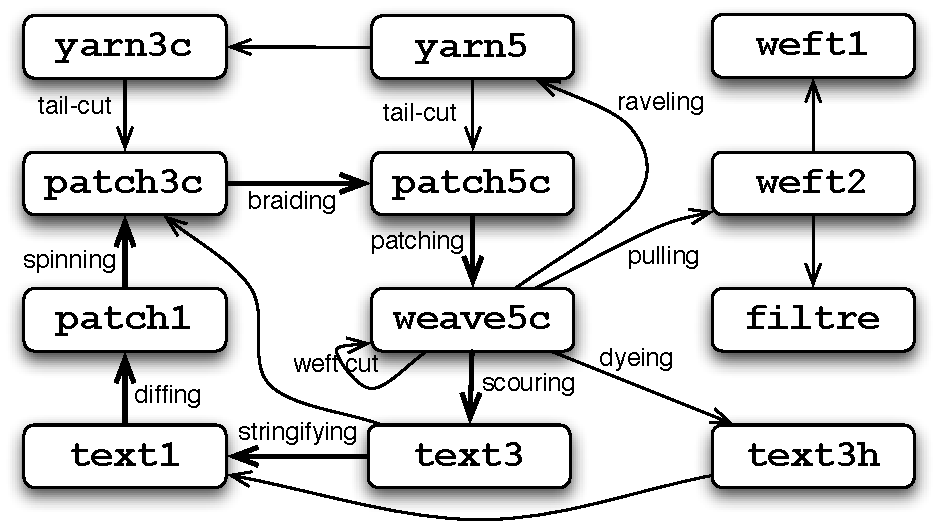
\includegraphics[width=0.48\textwidth]{operations.pdf}
\caption{Causal model formats and operations.} \label{fig:ops}
\end{figure}

\subsection{Scouring (weave to text)}
The central format of the model is {\tt weave5c}.
A weave might be transformed into {\tt text3} by \emph{scouring}: clearing weave of all the deleted atoms (immediately followed by a \bsp) and all the special symbols: \\
{\small \verb`s/(...(..))(`\bsp\verb`\2..)+|[`\bsp\zero\cnc\verb`].{4}|(.)..(..)/$4$5/g`}\\
Out of the atom's 5c-form, only the symbol and its id are taken, thus the output is a 3-form.
This regex is simplified for the ease of understanding; it ignores undeletions (see Sec.~\ref{sec:undo}).
%That is necessary , as PCRE is an étalon of ``write-only language''. 
The resulting {\tt text3} might be trivially \emph{stringified} into {\tt text1}, i.e. the text itself: {\small \verb+s/(.)../$1/g+}.

\subsection{Diffing (text to patch)}
The text is then put into the editor; the user makes some changes.
Those changes might be tracked either by listening to  basic events or by comparing text snapshots using diff and/or heuristics.
The result is a chain of {\tt patch1} substrings corresponding to inserted and removed spans of the text; their offsets in the original text are known.
That allows to check {\tt text3} for atom ids corresponding to the change: either attachment points for insertions or sets of removed ids for deletions.
Then, we may \emph{spin} {\tt patch3} and \emph{braid} a {\tt patch5c}, which contains the inserted atoms in their full 5c-form. 

\subsection{Patching (patch to weave)}
The {\tt patch5c} is then distributed to other users. Once it arrives, it should be integrated into their weaves.
First, it is split into causal blocks; one block is typically a causal chain of atoms corresponding to a period of uninterrupted typing.
A block has a single attachment point in the causal tree and might be inserted into the weave as a substring.
Its insertion point is just after the causing atom of the block's head/root atom, unless there is the case of unaware siblings which is addressed in Sec.~\ref{sec:unre}. Here I'll only add a safeguard by checking that the head atom is aware of the current right neighbor of its causing atom: \\
{\small \verb`s/^((?:.{5})*?)(...$C([`\bsp\cnc\verb`]$C..)*)(?=...($F))/$1$2$P/`}\\
This regex clearly needs explanation.
First of all, the regex is anchored to the beginning of the string to ensure it always matches with $\times 5$ offset and never across 5-form's atom boundaries.
Second, symbols \bsp~and \cnc~are supposed to follow their causes, see Sec.~\ref{sec:undo} for explanation.
Third, the regex includes three variables: \verb+$C, $F+ and \verb+$P+.
~\verb+$C+ is the atom id of the head's causing atom; \verb+$P+ is the inserted block; \verb+$F+ is an awareness {\tt filtre} of the head atom.
Filtre stands for ``filtering regex''; {\tt filtres} are produced from a {\tt weft2} by another regex, e.g. {\tt filtre('a2b4') = 'a[0-2]|b[0-4]'}.
A {\tt filtre} matches two-char atom ids that fall within the causal subtree cut by the {\tt weft2}.
Another common use for {\tt filtre} is to obtain a historical revision of a weave:  {\small \verb`s/(...($F))|.{5}/$1/g`}, which in turn may be scoured to get a historical revision of the text.
In the case of patching, we produce a {\tt filtre} out of the head symbol's awareness {\tt weft2} just to ensure the author of the head symbol was aware of the symbol to the right (no unaware siblings).

\subsection{Patching with unaware siblings} \label{sec:unre}

Well, what if unaware siblings are introduced by other users, so the first method of patching fails?
This is exactly the situation to apply Lemma~\ref{lemma:1}. 
We single out the causal block of the heads's causing symbol, then we split it into causal blocks of the head's siblings, then we insert our block between its sibling causal blocks, according to the {\tt weftI} ordering (see Sec.~\ref{sec:siblord}).
The implementation of this case is less straightforward.
While still relying on regular expressions, it involves some ``manual'' work and, most importantly, the costly operation of \emph{pulling} (awareness weft derivation), which does several passes of the weave (see Sec.~\ref{sec:pulling}).
The assumption is that concurrent insertion of symbols at the same position in the text is a rare event, so this non-trivial machinery will be invoked ``once a year''.
It should be noted that the simpler no-unaware-siblings patching algorithm employs awareness wefts as well.
Luckily, in that case wefts might be cached and incrementally updated due to append-only nature of yarns, so the costly recalculation is unnecessary.

\subsection{Pulling awareness wefts} \label{sec:pulling}

The operation of \emph{pulling} derives an awareness weft of an atom.
As an atom id is a trivial {\tt weft2}, pulling might be seen as transitive closure of the awareness relation.
Technically, pulling is a cycle of (a) extracting all atoms from a weave that fall under a weft and (b) using their ids to build the next iteration of the weft.
A string of concatenated ids is technically a {\tt weft2}, but it has lots of redundancy.
Such watery wefts are \emph{dried} into non-redundant form by a reverse filtre that matches everything but the latest id in every yarn:
{\tt revfiltre('a1a4b2') = \verb+'a[^1-∞]|a[^4-∞]|b[^2-∞]'+}.\\
Once two consecutive iterations produce the same weft, the closure has converged.
Making numerous passes of the complete weave might be costly.
For efficiency reasons, pulling is done using a condensed form of a weave named {\tt deps4}; it only contains atoms that reference other yarns.
If an atom is caused by another atom on the same yarn, it does not affect the result of pulling. 


\subsection{Scouring (with undo and shortcuts)}	\label{sec:undo}
The undo function boils down to deleting all insertions and cancelling all deletions that happened after some recent weft.
The cancelling is done by the \cnc ~symbol, which is a ``deletion for deletions'';~\cnc ~recovers its causing symbol, by cancelling all deletions it is aware of.
The introduction of the symbol is mostly a technical optimization to allow for bulk processing of deletions and undeletions. 
Differently from insertions, \bsp ~and \cnc ~do not form causal chains naturally and processing a thousand of \bsp ~one by one might be time-consuming.
In general, the regex implementation employs several shortcuts to improve performance.
It is good as long as the final result (the text) matches the definitions of Sec.~\ref{sec:textile}.
Special symbols are most heavily ``shortcut'' as they do not show up in the resulting text.
As an extreme example, \zero ~does not affect any operation but the pulling, and pulling does not depend on atom order.
Just to get \zero's out of the way, they are appended after \eoa.
All \bsp ~and \cnc ~stick to their causes as (a) they interact with their cause only, (b) they cause nothing but \zero ~and (c) their precise order is irrelevant.
All \cnc ~prepend every \bsp ~they cancel; thus, a {\tt weave5c} might have  several copies of a single \cnc, in case it cancelled multiple \bsp.
Another bulk-processing shortcut is that under certain conditions spans of \bsp ~and \cnc ~may share the same id.
%They have no children, so their actual id is not that useful.
As we may see, the difference between theory and practice truly exists in practice.
Thus, the full scouring regex is: \\
{\small \verb`s/.{5}(?:(?:`\cnc\verb`.{4})+`\bsp\verb`.{4})*`\bsp\verb`.{4}(?:[`\bsp\verb``\cnc\verb`].{4})*|\`\\
\verb`.0.0.(?:[`\bsp\zero\cnc\verb`].{4})*|`\verb`(.)..(..)(?:[`\bsp\verb``\cnc\verb`].{4})*/$1$2/g`}\\
Quite nicely, it now lacks backreferences and thus friendly to DFA/NFA-based regex engines~\cite{re2}.

\subsection{Misc operations}

So, we went through the full cycle: from a weave to a text to a patch and back to the weave.
Other operations are less critical for the understanding of the model.
For example, the operation of \emph{dyeing} derives a {\tt text3h}, which is a ``painted'' text in a special 3-form showing the difference between two revisions. 
Namely, instead of the standard (yarn id; symbol id) pair, a symbol is followed by a pair of yarn ids: one for a yarn that inserted that atom, another for a yarn that removed that atom.
If no such change happened between the two revisions, then id is null.
The {\tt text3h} string may then be transformed into highlighted text or HTML.

%The operation of saving is only supposed to signal the author's awareness/acceptance of certain revision.
%Physical ``save'' to the permanent storage happens automatically once atoms are appended to yarns and broadcasted; there is no way to revoke atoms.
%Thus, save is done by  adding \zero ~atoms caused by the tail atoms of all known yarns.

A solid slice of RCS functionality is dealing with branches, i.e. parallel versions of the same text/source.
In a causal tree, a branch in the RCS sense corresponds to (literally) a set of branches.
Those branches may be attached or detached on request.
Storage-wise, branches might be either tails of certain yarns cut off by a weft or entire special yarns.
Branches may host parts of a text with special access rights, overlay modifications (notes, annotations, bubbles/balloons), pending/discussed draft modifications or just scratchpad remarks.
As long as the point of attachment still exists in the text, a branch might be cleanly attached.
Otherwise, it is attached ``uncleanly'' into approximately the same place.
Differently from the diff-patch paradigm, the process does not depend on mutations of the context, demands no heuristics, combinatorics or manual intervention. Changes are detachable and, generally, more manageable, as CT tracks each symbol's origins and dependencies.

To summarize, the model now implements all the basic functions of a revision control system in a simple, portable and truly decentralized way.

\section{Estimations} \label{sec:estim}

Once basic data structures and algorithms of the model are explained,
it is time to consider practical feasibility of the introduced model.
It is definitely impossible to foresee every difficulty implementors may face, so this section will focus on fundamental limitations introduced by the model itself.
Section \ref{sec:formats} addresses the limits of the atom format.
Section \ref{sec:weave-growth} analyzes weave size evolution in time, using Wikipedia articles as reference data.
Section \ref{sec:io} discusses input-output (I/O) patterns of data structures used.
Section \ref{sec:sec} applies the CT model to hierarchically structured text.

\subsection{Limits of atom-based formats} \label{sec:formats}
First source of risk is the CPU time necessary to process such a fine grained change/history format.
With regular expressions, all the operations listed in Section~\ref{sec:algos} run in negligible time even on bigger texts. 
If ran within a browser, $O(N)$ regular expression passes a 1MB string in around a millisecond.
The patching operation for the case of unaware siblings may take more time, let it be 100ms, but it is supposed to be a rare ``once a year'' case.
The overall computational cost of assembling a weave from source yarns using regexes is $O(N^{2})$, i.e. a combinatory explosion is possible, unless the weave is cached.
In the latter case, $O(N^{2})$ accumulates historically, over the years of the text's lifetime.

Another risky trick is using Unicode chars as, essentially, numbers.
In fact, common regular expression engines reliably support only the first 50,000 code points or, more precisely, the [U+0,U+D800) interval. 
In case a single author generates more than 50K of symbols, that author should be assigned an additional yarn id.
In total, the capacity of this numbering system limits text size to $2,5\times10^9$ symbols, which is more than enough; three volumes of ``War and Peace'' in Russian take less than 0.1\% of that, 2,56MB in UTF-8. 
The 50,000 code points limitation also limits the number of yarns and, correspondingly, coauthors of a single document.
Practically, it is hardly a problem, as even the most popular project, namely Wikipedia, has only three articles with an author count above $2^{15}$: the Introduction, the Sandbox and the Archive of the Sandbox, i.e. pages every new user predictably bumps into.
Excluding the exercise, complaint and similar pages, the topmost ``real'' page has an author count of 13680 as of the 2009-08-16 snapshot.
That is the ``George W. Bush'' article and the reasons for the high author count are likely to be similar to the Sandbox case.
In case CT will be used for crowdsourcing a world population census or similar purpose, there are three possible workarounds: (a) use two Unicode chars instead of one; (b) use regex engines that support $2^{32}$ character range or (c) split giant texts into smaller texts or sections (see Sec.~\ref{sec:sec}).

\subsection{Weave growth}	\label{sec:weave-growth}

The size of a text is not of big concern, as texts are small in general: the mass of Web traffic is dominated by images, not to mention video content.
The entire Web in text-only indexed form fits into a single NAS server~\cite{own-experience}. What actually makes web search companies to build giant facilities is the volume of simultaneous search requests.
But a weave holds the entire text's mutation history, so it may be substantially bigger than the plain text itself.
Although, for practical everyday use, full weaves are not necessary, as the user is more likely to be interested in the changes since the last visit, not the full mutation history.
Thus, some distilled version of a weave may be used, long-dead parts being {\tt filtre}d out.
Another general consideration is that the amount of processed information (think of the Web) tends to grow exponentially. Due to $\int e^{cx}dx \sim e^{cx}$, the mass of the last revision is likely to differ from the mass of the full history (i.e. weave) just by some factor (which might be big).
As the saying goes, ``devil is in the details'', so let's consider the actual numbers.

\begin{figure} 
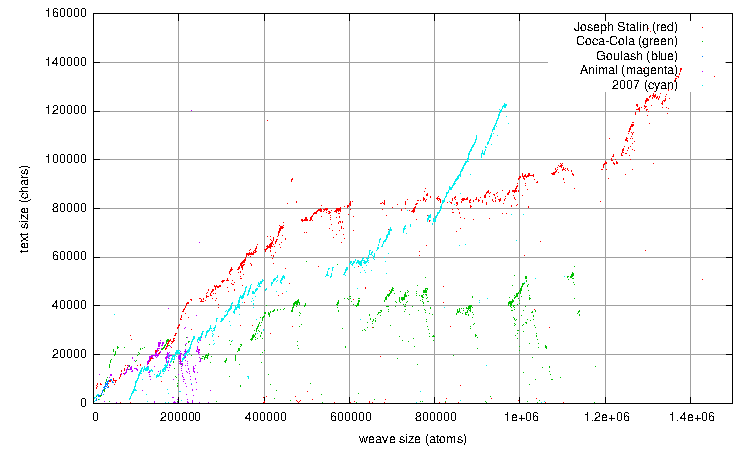
\includegraphics[width=0.48\textwidth]{weave-growth.pdf}
\caption{Weave size evolution experiments.} \label{fig:weave}
\end{figure}
\begin{figure} 
\resizebox{0.48\textwidth}{!} {
\begin{tabular}{|c|r|r|r|r|r|r|}
\hline
Article & snapsh. & .gz & .7z & {\tt weave5c} & {\tt text1} & git \\
\hline
Coca-Cola& 254Mb &78.4Mb & 482Kb & 1.13Ma & 52Kc & 9.25Mb\\
J. Stalin&754Mb& 281Mb&891Kb& 1.38Ma&137Kc& 10.6Mb\\
Goulash&2.2Mb&45Kb&26Kb&46Ka&8.6Kc& 348Kb\\
Animal & 69.9Mb & 1.1Mb & 252Kb & 254Ka & 28Kc & 3.45Mb\\
2007 & 609Mb & 191Mb & 782Kb & 967Ka & 122Kc & 10Mb\\
\hline
\end{tabular}
}
\caption{Space consumed by full-history storage in misc formats; postfix ``b'' stands for bytes, ``c'' for Unicode chars (1-2 bytes, depending on charset and encoding), ``a'' for 5-form atoms (5-10 bytes).} \label{fig:sizes} % Megabytes are decimal.
\end{figure}

To estimate growth dynamics and overhead of a weave, I plotted weave size evolution for five Wikipedia articles of different classes (se Fig.~\ref{fig:weave}), using the January 2008 enwiki dump.
The articles used were ``Coca-Cola'' (popular), ``Joseph Stalin'' (popular, big, controversial), ``Goulash'' (obscure), ``Animal'' (popular, term), ``2007'' (popular, big, year).
%Weaves were derived from the full history dump dated January 2008.
The first finding is that article evolution depends a lot on the human factor, e.g. the ``editorial pressure'' keeping the article size within bounds.
The second finding was that the rate of vandalism is fairly high.
Vandalism had to be filtered out as it arbitrarily inflates sizes of the weaves, e.g. if the entire text is deleted and recovered back, or megabytes of garbage are pasted into the article.
Namely, all changes that were rolled back within 20 revisions were  not counted.
Fortunately, separating cases of vandalism and edit warring from article refactoring and well-intentioned edits is out of scope of this article.
While the simple criteria left some vandalism undetected, it was good enough to see the trends.
%I assume that large gaps in the graph correspond exactly to undetected vandalism cases (weave size increased abruptly, text size stayed in place).
During periods of unconstrained growth, weave size grows (roughly) linearly with the number of edits, as well as the article size.
But, there is also editorial pressure that keeps the article size within bounds. Sometimes, an article gets refactored and even shrinks.
What is relevant for us is the general correspondence between space requirements of different full-history text storage formats.
I have compared six formats: bare snapshots, gzip and 7zip of snapshots, {\tt weave5c}, plain text of the last revision (no history) and a git repository keeping the entire history (measured immediately after \verb+git gc+, i.e. compression and garbage collection), see Fig.~\ref{fig:sizes}.
As a rule of thumb, \emph{full} weave size may be estimated as x100 the plain text size.
Mass of a pre-filtered weave is likely be around text size times 5 or 10, depending on charset/encoding, which factor is defined by the form-5 overhead.
Interestingly enough, a gzip of snapshots is far worse than an uncompressed weave.
A 7zip archive is better off, its main shortcoming being high CPU consumption. It took around 20 seconds to 7zip-unpack some of the articles, which makes the format  suitable for backup purposes only.

As a conclusion, the space efficiency of {\tt weave5c} as a versioned text format is comparable to the space efficiency of a git repository storing the same page history.
Thus, {\tt weave5c} is effective as a server-side versioned text format, although vandalism better be cleared, as it may arbitrarily inflate the overhead.
For sending to the client side, a weave better be prefiltered to keep only those changes of interest.


\subsection{I/O patterns}	\label{sec:io}

Finally, as we talk about data storage formats, it is definitely useful to consider their I/O patterns.
A weave is convenient for reading and processing, which is done in sequential passes.
It is much less convenient for writing, as it needs to be overwritten entirely after any modification.
A yarn is exactly the opposite: it is append-only, so writing is cheap, while reading and weaving together many yarns is both CPU and I/O consuming operation.
In practical scenarios, combined solutions might be better.
As an example, consider the {\tt weave5c+patch5c+text1} set.
Read-only clients may be served with {\tt text1}.
All ongoing modifications might be appended to {\tt patch5c}, which thus acts as a write cache.
The {\tt weave5c}, once read from the disk, should be immediately  updated with the {\tt patch5c}.
Once {\tt patch5c} becomes too big, the weave might be overwritten with its current version, {\tt patch5c} is thus emptied.
Other mixes are also possible, depending on trade-offs.
For native (non-regex) implementations, tradeoffs might be different; e.g. a {\tt weave5} might be assembled from a set of {\tt yarn3c} in log-linear time; as yarns are append-only they are also perfectly cacheable, etc etc.

\subsection{Sectioned model}	\label{sec:sec}

The causal trees model exclusively considers plain/flat text; formatted text is often modeled as a tree structure, e.g. HTML's Document Object Model (DOM)~\cite{dom}.
I will sketchily address this concern.~\footnote{My understanding of what should and what should not be done here is based on the experience of building a chain of prototypes over the past years~\cite{www06,csr07,wikisym08}.} 

While DOM imposes hierarchical structure on formatted text, the text per se was not historically considered hierarchical, except probably for its bigger units, i.e. \emph{sections}. 
As an example, remember LaTeX, the RFC text format, the wikitext or even the early pre-DOM HTML: the text is considered to be a flow of words and markup elements, the only hierarchically structured parts are sections/subsections.
Even browsers, as a matter of fact, start parsing with the ``tag soup'' model, later applying heuristics to transform it into an orderly tree. 

Note the open possibility to handle units of text hierarchical structure (sections) separately.
While each section might be considered flat in the pre-DOM HTML sense, different sections might reference each other through transclusion links thus forming a hierarchical structure.
Each section has its own weave. A weave is just a string, so the resulting data structure is simple enough.
As a result, we have a digraph of sections; that keeps the complexities of the document's hierarchy and revision control orthogonal. 
The sectioned structure allows to preserve histories once a section is moved within a document or even between documents.
With equal ease, it allows to prune old history once an article is refactored.
Removed sections are still mentioned in histories of their parent sections, so historical revisions of the whole document can be recovered. At the same time, long-dead parts do not clutter the weaves currently in use.
Last but not least, the sectioned structure allows to relax the 50,000 authors limitation: a single section might not have 50K symbols, not to mention authors.

Back to HTML, the correct XHTML structure cannot be guaranteed when merging concurrent modifications. For example, two overlapping tag ranges cannot be merged correctly in the general case, e.g. 
{\small \verb+<i>Quick <b>brown</i> fox</b>+. }\\
That of course returns us to the tag soup situation; but that is the state of the things anyway and  browsers are good in dealing with it. 
Once the correct hierarchical structure of the text is ensured by the structure of (isolated) sections, best-effort merge of decorative tags within sections may be offloaded to the browser.
In either case, this alternative seems more practical than distributed real-time revision control of DOM trees (see Sec.~\ref{sec:waveot}).


\section{Related work} \label{sec:reflections}

The model itself, its data formats and algorithms are now fully described, so we may compare them to the relevant work in the field.
Not to limit ourselves to feature-by-feature comparisons, I will put the CT model into a broader context to uncover similarities and dependencies that have a chance of being useful or insightful.

\subsection{Operational Transformation} \label{sec:ot}

The causal model fulfills three requirements of the OT CCI correctness model (see Sec.~\ref{sec:siblord} for one-paragraph proof).
%Causality preservation holds by design, as an atom is never introduced to the weave before all any of the atoms it is aware of.
%Convergence is insured as the order of atoms in a weave does not depend on the order of arrival.
%Intention preservation, in the sense of applying changes to a wrong position in the text, is trivially solved: the logic is not positional.
Compared to the mainstream OT, the use of unique atom identifiers and  ordering of atoms into a tree removed all the arcane complexity of position-dependent operations and transformations.
That complexity was mostly caused by the relativistic nature of distributed systems, where the perceived time and order of events varies for different observers.
Using relativistic analogies, the CT construct resembles the light cone (aka Minkowski spacetime) approach to understanding order and causality of events.
Instead of reshuffling basic events that happen at different times at different points in space, as perceived by different observers, the CT model considers the entire \emph{static} geometric shape in spacetime.
As a consequence, quite differently from operational transformation schemes, causal trees absolutely lack the transformation aspect: atomic operations stay intact and interact in simple predictable ways.

\subsection{Post-OT schemes}
The reliance on atom ids makes CT similar to the WOOT~\cite{woot} transformationless OT scheme that also abandons positional logic in favor of unique atom identification.
While WOOT records both left and right neighbors of a newly introduced atom, CT records just one (the ``cause''). 
In some situations, indeed, CT has to mention the second neighbor using the \zero ~atom, but that is an exception.
WOOT avoided using vector clocks, based on the assumption that the size of a vector is proportional to the total number of participants.
But in the scope of a single page or a section the number of editors is manageable. Vector clocks (wefts) also turn to be quite handy as revision identifiers. \\
As well, CT has some similarities to another post-OT system named Logoot~\cite{logoot}.
Logoot's list-identifiers can be compared to concatenations of CT ids along the path from the root to the atom.
In CT, this structure is used implicitly.
Logoot takes some measures to avoid accumulation of tombstones (i.e. deleted historical content). That is mostly caused by its reliance on line-based granularity of change tracking, which exaggerates the overhead of history-keeping, in case small changes are prevalent.
Tombstone avoidance is much less relevant for symbol-based revision control.
CT follows the DRCS principle of each repository being an independent peer hosting the entire known history.
In this context, Logoot's history elimination is unacceptable. \\
Regex-based implementation is an absolutely unique feature of CT, not ever attempted in OT or post-OT or any other kind of revision control framework.

\subsection{Xanadu}

There are some parallels between CT and the historical Xanadu hypertext model.
The spirit of Xanadu is to keep all the versions of all texts at the same time, by clearly separating the original input from the actual revisions of the text~\cite{xanacarpet}.
A very similar  approach is seen in causal trees: primary input is put into yarns, while all the actual revisions are subsequences of the weave.
The Xanadu objectives of ``origin connection'', ``side-side intercomparison'', ``deep version management'' and ``incremental publishing'' are addressed in CT.
Still, the implementation is very different.

\subsection{Lamport-Fidge vector clocks} \label{sec:lamport}

The causal tree model perfectly matches the entities of the Lamport--Fidge~\cite{lamport,fidge} vector/logical clocks model.
Namely, a yarn corresponds to a process, foreign causality relations - to messages, yarn offsets to local logical clocks and wefts to vector clocks. 
Awareness order follows the lines of Lamport's synchronized logical timestamps.
The weft order is similar to Fidge's vector clock ordering, but there are no strict equivalence here.
Interestingly, the Fidge-Lamport model was inspired by the special theory of relativity.
In this article, we always observed a causal tree from a certain \emph{frame} of reference (see Sec.~\ref{sec:data}) centered at a certain yarn.

\subsection{Distributed wikis}

The first distributed wiki proposal was made by Ward Cunningham, the original inventor of wikis~\cite{folk-memory}.
Numerous peer-to-peer/distributed/federated wiki proposals and prototypes were made since \cite{www06,buraga,distriwiki,concerto}, but none crossed the critical robustness/usability threshold to reach any notable acceptance. Probably, a simpler distributed revision control technology will make some advance here.

Currently, Wikipedia faces scaling problems~\cite{wp-decay,no-singularity}; nature of those problems is quite complicated and cannot be addressed in this article.
Some research effort was put into engineering a decentralized Wikipedia based on Distributed Hash Tables (DHTs, ~\cite{urdaneta}).
That is merely a technical decentralization that addresses possible funding shortages.
Another side of the problem is social decentralization.
How to prevent turf wars and contributor alienation?
Is it possible to create multiple competing pedias?
How could we possibly test novel forms of contributor organization and incentivization?
Will the inclusionist approach work, i.e. could we use Wikipedia for specialized knowledge?
My honest belief is that decent distributed revision control technology is absolutely necessary just to start thinking about those questions.

Eventually, decentralized version control with easy forking and easy merge of branches may lead towards the vision that Linus Torvalds has explained as ``crosspollination and natural selection''~\cite{linus-pollinates} in application to the Linux development.
Currently, those ideas are manifested in the design of the git RCS.
Unfortunately, the git is not Web-ready.
It is precisely fit for its current purpose and it was never intended to run in a browser or to be simple enough, etc.
Empowering the regular user with the advanced collaboration and revision control toolset might be a worthy objective.


\subsection{Google Wave}  \label{sec:waveot}

Google Wave relied on a flavor of Operational Transformation for
real-time version control. The enhanced OT flavor is supposed to
handle both plain text and tree-like XML DOM structures.
Informally, the main problem of the resulting technology is that
its complexity is OT complexity \emph{times} XML complexity. 
The authors even had to enrich XML with additional entities 
named ``annotations'' to make it suitable for their needs.
There are 15 sorts of different mutation operations used in Wave
OT, some as opaque as ``delete anti-element end''~\cite{waveot}.
Theoretically, the potential for unexpected feature interactions
tends to grow combinatorially with the number of primitives.
In practice, the overcomplication resulted in numerous bugs and
slow unresponsive user interface~\cite{own-experience}.
According to an insider~\cite{gerasimov}, in 6 months since the
projects's launch the possibility of working with partial
histories is not  implemented yet; pages are bootstrapped with
their complete histories. 
%Compare that to the ease of applying a filtre to a weave in the CT model.


\section {Conclusion} \label{sec:conclusion}

%While many previous revision control technologies were either fully distributed or real-time or Web-based, the causal trees combine all that at once.

The CT model makes four main contributions. First, it allows to implement first-class real-time collaborative editing in the browser (as in Google Docs). Second, it allows that not only in a client-server setting, but in a network of any topology. That enables highly decentralized workflows (like in git). 
On the technical side, the third contribution is a simple string-based format for versioned text and trivially portable regex-based algorithms. 
That enables the fourth contribution which is the deep hypertext capability with instant access to every prior version of a document, per-character authorship information, real-time difference between any two versions and attaching/detaching of branches.
The fourth one is the most hard to estimate, as there is nothing yet to compare it to.
%causal trees are able of making the critical step from an application to an open format used at mass scale in highly distributed highly heterogeneous environment, which is the Open Web.


\section{Acknowledgements}

Many thanks to M.V. Volkov, B. Cohen, A. Pronchenkov, S. Pupyrev, N. Andrade, A. Iosup and J. Gerber for priceless feedback that influenced this paper. 
\bibliographystyle{plain}
\bibstyle{plain}
\small
\bibliography{sources}

\end{document}
